\documentclass[a4paper,12pt]{article}
\usepackage{HomeWorkTemplate}
\usepackage{circuitikz}
\usepackage[shortlabels]{enumitem}
\usepackage{hyperref}
\usepackage{tikz}
\usepackage{amsmath}
\usepackage{amssymb}
\usepackage{tcolorbox}
\usepackage{xepersian}
\usepackage{mathtools}
\settextfont{XB Niloofar}
\usetikzlibrary{arrows,automata}
\usetikzlibrary{circuits.logic.US}
\usepackage{changepage}
\newcounter{subproblemcounter}
\setcounter{subproblemcounter}{1}
\newcommand{\problem}[1]
{
	\subsection*{
		تمرین
		#1
		}
	\setcounter{subproblemcounter}{1}
}
\newcommand{\subproblem}{
	\textbf{\harfi{subproblemcounter})}\stepcounter{subproblemcounter}
}


\begin{document}
\handout
{مباحث ویژه در سیستم‌های دیجیتال}
{دکتر ایمان غلام‌پور}
{نیم‌سال اول 1400\lr{-}1401}
{اطلاعیه}
{امین کشیری}
{۹۷۱۰۱۰۲۶}
 {توضیحات پروژه}



\section{مقدمه}
در این پروژه، با استفاده از ایده‌ها و روش‌های مختلفی که در طول ترم آموختیم، 
اطلاعاتی را از داده‌ها بیرون کشیدم. بخش‌های مختلف این پروژه را در فایل‌های 
jupyter
جداگانه قرار داده‌ام، و توضیحات هر بخش را نیز جداگانه در این فایل نوشته‌‌ام. 


\subsection{توضیحات کلی}

\begin{enumerate}
	\item 
	در ابتدای تمامی کدها تنظیمات اولیه اسپارک را انجام دادم، و سپس فایل 
	csv
	داده شده را 
	load
	کردم. 

	\item 
	در بعضی از بخش‌ها، روز ۸م را از داده‌ها حذف کردم. دلیل این کار این بود از تمامی روز‌ها
	به اندازه‌ی متناسب با هم داده داشته باشیم. در غیر این صورت تعداد داده‌ها از روز سه شنبه 
	دو برابر باقی روز‌ها می‌شد. کار‌های دیگری نیز می‌توانست انجام بگیرد. مثلا می‌شود داده‌های روز سه شنبه را 
	میانگین بگیریم (
		یعنی در تمام قسمت‌هایی که تعداد متغییری را شمر‌ده‌ایم، برای روز سه شنبه این تعداد را 
		تقسیم بر ۲ کنیم
	). 
	در بعضی از قسمت‌ها اما این زیادتر بودن داده‌های روز سه شنبه مشکلی ایجاد نمی‌کرد. اما دقت 
	کنید که در بعضی‌ از قسمت‌های دیگر می‌تواند تحلیل ما را دچار انحراف کند (
		مثلا ممکن است به اشتباه نتیجه‌ بگیریم که روز سه شنبه روز پر تردد تری است، یا 
		دوربین‌هایی که در روز سه شنبه دیده‌ می‌شوند را به اشتباه مهم تر در نظر بگیریم
	). 

	\item 
	توضیحات کد و روند اجرا را در فایل‌های 
	jupyter
	نوشته‌ام. سعی کرده‌ام که توضیحات منطق پشت کد‌ها را در این مستند بنویسم (
		و نه در خود کد‌ها
	). 
	بنابرین توضیحات تکنیکال خود کد در اینجا کمتر نوشته شده است. 
\end{enumerate}


 
\section{General}

\section{Clustering}

\subsection{توضیحات کلی}

با استفاده از خوشه‌ سازی، سعی کردم دوربین‌ها را به دسته‌های مختلفی تقسیم کنم، و برای 
هر دسته مفهومی بیابم. نماینده‌ هر دوربین در این روش، یک بردار با اندازه‌ی 
$24 \times 7$
است، که در هر خانه‌ی آن تعداد تردد در آن ساعت از روزهفته قرار گرفته‌است. ۲۴ ساعت اول 
برابر با یک‌شنبه است، ۲۴ ساعت بعدی برای دو شنبه و الی آخر. پس بردار 
متناظر هر دوربین، تعداد تردد‌ها در هر ساعت از یک هفته را برای آن دوربین 
مشخص می‌کند. 

برای خوشه‌سازی از الگوریتم 
LDA یا 
\lr{Latent Dirichlet Allocation}
استفاده شده است، که همانطوری که در درس دیدیم استفاده اولیه آن پیدا کردن 
توزیع 
topic
های مختلف و کلمات آن‌ها برای هر مقاله است. با استفاده از این الگوریتم برای 
داده‌های تردد ماشین‌ها نیز می‌توانیم دقیقا به چنین توزیعی برسیم. 

یکی از متغییر‌های بسیار مهم در این بخش، 
\lr{cluster\underline{ }center}
است، که تعداد کلاستر‌های نهایی را مشخص می‌کند . با تغییر این متغییر این متغیر می‌توانیم تعابیر متفاوتی از داده‌ داشته باشیم. اما یکی از واضح‌ترین نتیجه‌‌ها برای
\mbox{\lr{cluster\underline{ }center = 3}}
به دست می‌آید که آن را در شکل‌های زیر می‌بینید: 

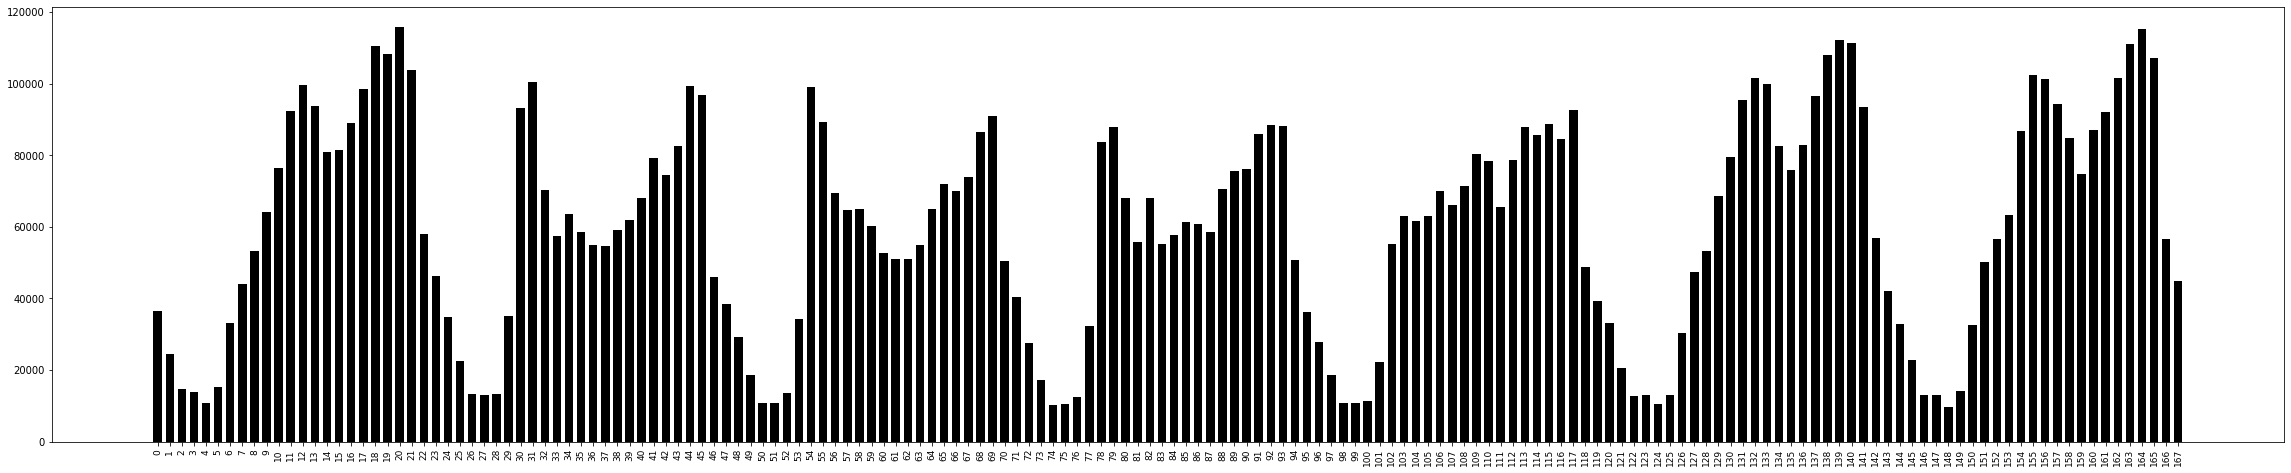
\includegraphics[scale=0.2]{images/clustering/1.png}

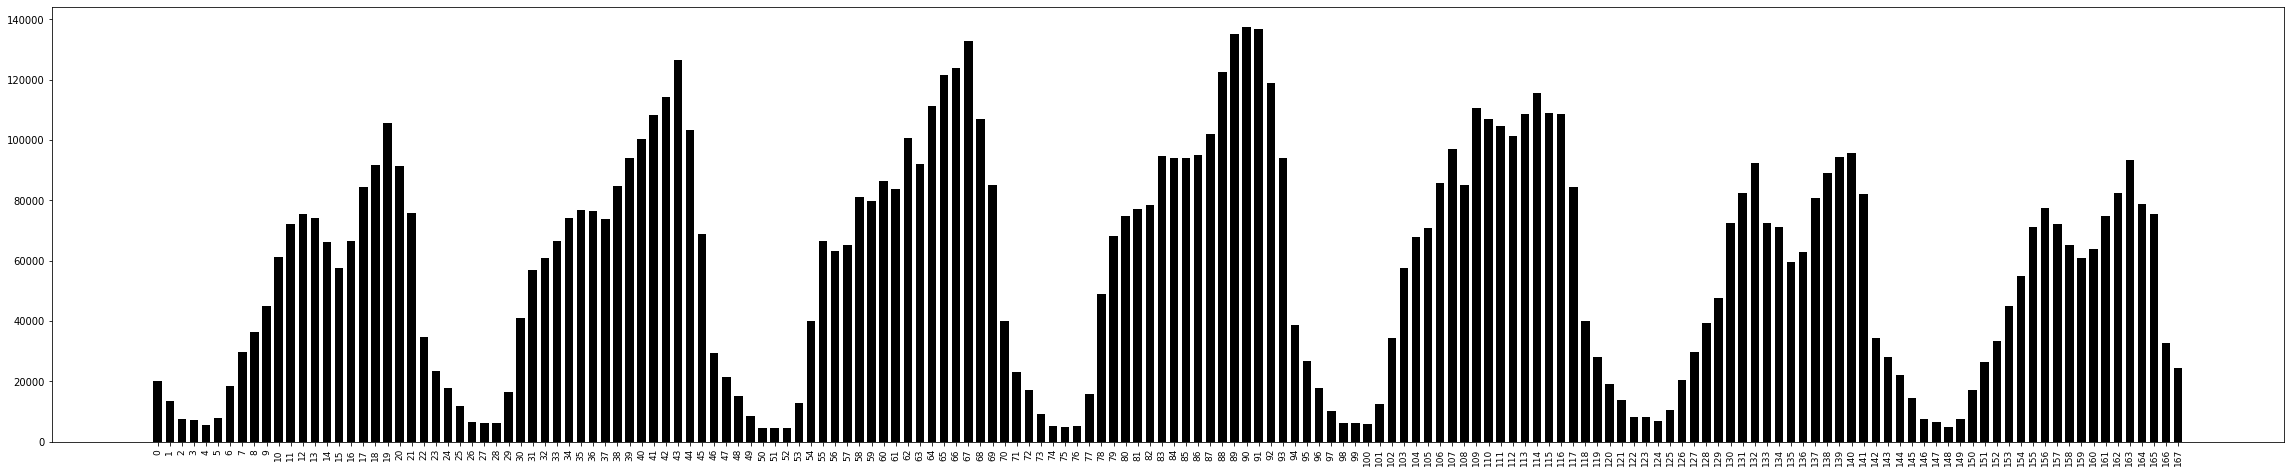
\includegraphics[scale=0.2]{images/clustering/2.png}

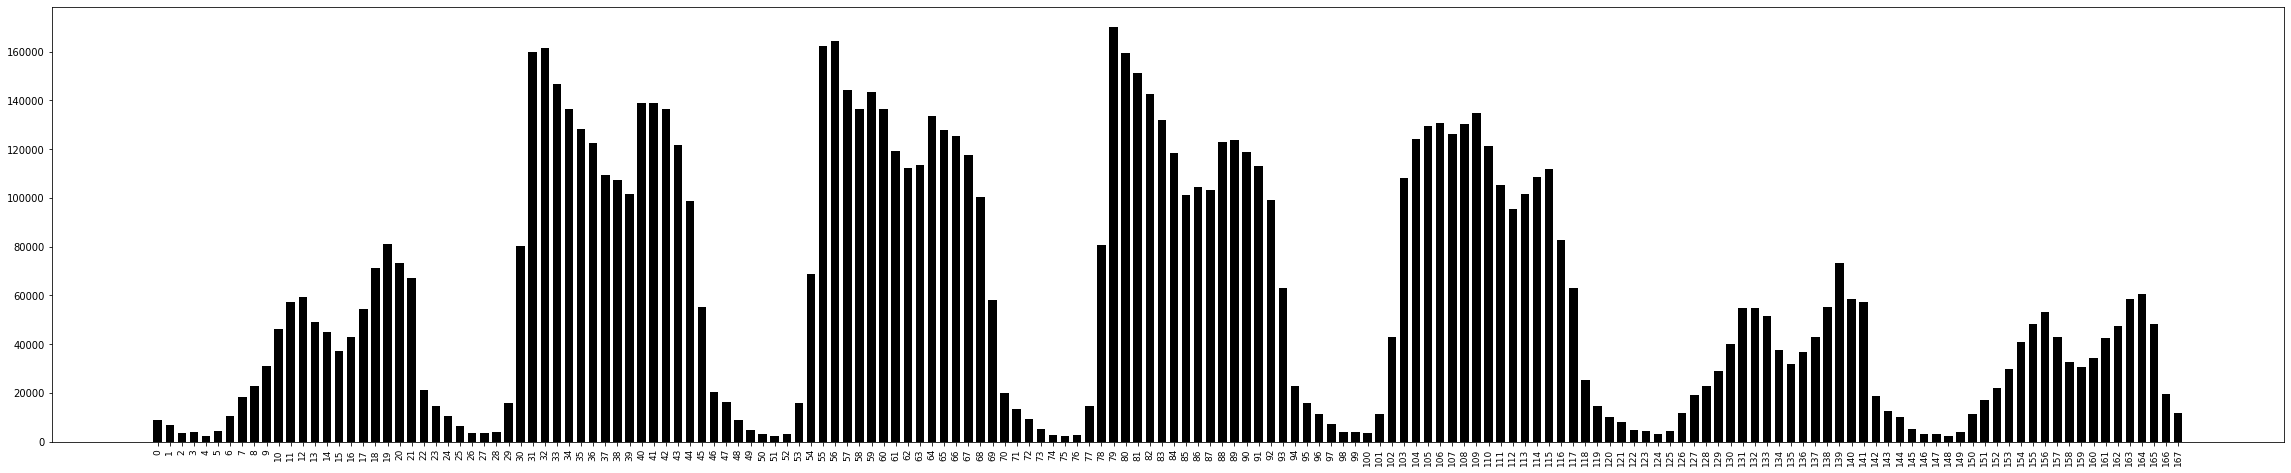
\includegraphics[scale=0.2]{images/clustering/3.png}


\subsection{تحلیل نتایج}

مهم‌ترین نکته‌ی این سه تصویر، روند تغییر تردد‌ها در هر روز است. در دسته‌ی اول، 
تردد در ساعات اولیه روز افزایش می‌یابد، در هنگام ظهر کاهش پیدا می‌کند، سپس دوباره در 
شب افزایش پیدا می‌کند. در دسته‌ی دوم، تردد در صبح کم است، اما کم کم افزایش می‌یابد و در شب 
به اوج خود می‌رسد. دسته‌ی سوم روندی دقیقا عکس دسته‌ی دوم دارد، و بیشترین تردد را در صبح 
دارند و سپس کاهش می‌یابد. 

سه دسته‌ی بالا را می‌توانیم به این صورت تفسیر کنیم. دسته‌ی اول نقاط پر تردد شهر هستند، که هم در روز 
و هم در شب تردد بالایی دارند. این نقاط احتمال مکان‌هایی وسط شهر هستند که تمام 
طول روز تردد دارند ( البته طبیعتا تردد در ظهر کاهش می‌یابد). 
دسته‌ی دوم، احتمالا مکان‌های دیدنی و تفریحی و یا بازار‌های شبانه هستند 
که در طول روز تردد زیادی ندارند (به دلیل این که مردم مشغول کار و مدرسه و ... هستند). 
دسته‌ی سوم نیز احتمالا مکان‌هایی هستند که در طول روز تردد بالایی دارند، مانند مکان‌های اداری، مسیر مدارس و ادارات، یا دوربین‌های نزدیک به مثلا نانوایی‌ها. 

یک نکته‌ی بسیار جالب دیگری که در این تصاویر دیده می‌شود، این است که که تردد 
در روز‌های جمعه، شنبه و یک شنبه به طرز جالبی پایین است. با چک کردن این ۳ روز روی تقویم، فهمیدم که این روز‌ها 
تعطیل رسمی بوده‌اند (قیام ۱۵ خرداد و شهادت امام جعفر صادق (ع)). بسیار جالب است که این کاهش 
ترددها، فقط در دسته‌ی سوم رخ داده‌است، که دقیقا با شهود ما همخوانی دارد، که دسته‌ی سوم مکان‌هایی 
مانند مدارس و ادارات هستند. همچنین، الگوی کاهشی تردد در این سه روز از بین رفته‌ است 
که باز هم مطابق با الگوی پیدا شده است. 

\section{Pixie}



\section{HITS}

\subsection{توضیحات کلی}

کدهای ابتدایی این قسمت بسیار شبیه به حالت‌های قبلی هستند. در این الگوریتم، 
دوربین‌ها به عنوان
hub
 و زمان‌ها به عنوان 
auhtority
در نظر گرفته‌شده‌اند. سپس با استفاده از تجزیه‌ی 
SVD
الگوریتم 
HITS
را پیاده‌سازی کردم. نتایج نهایی به صورت زیر بودند: 

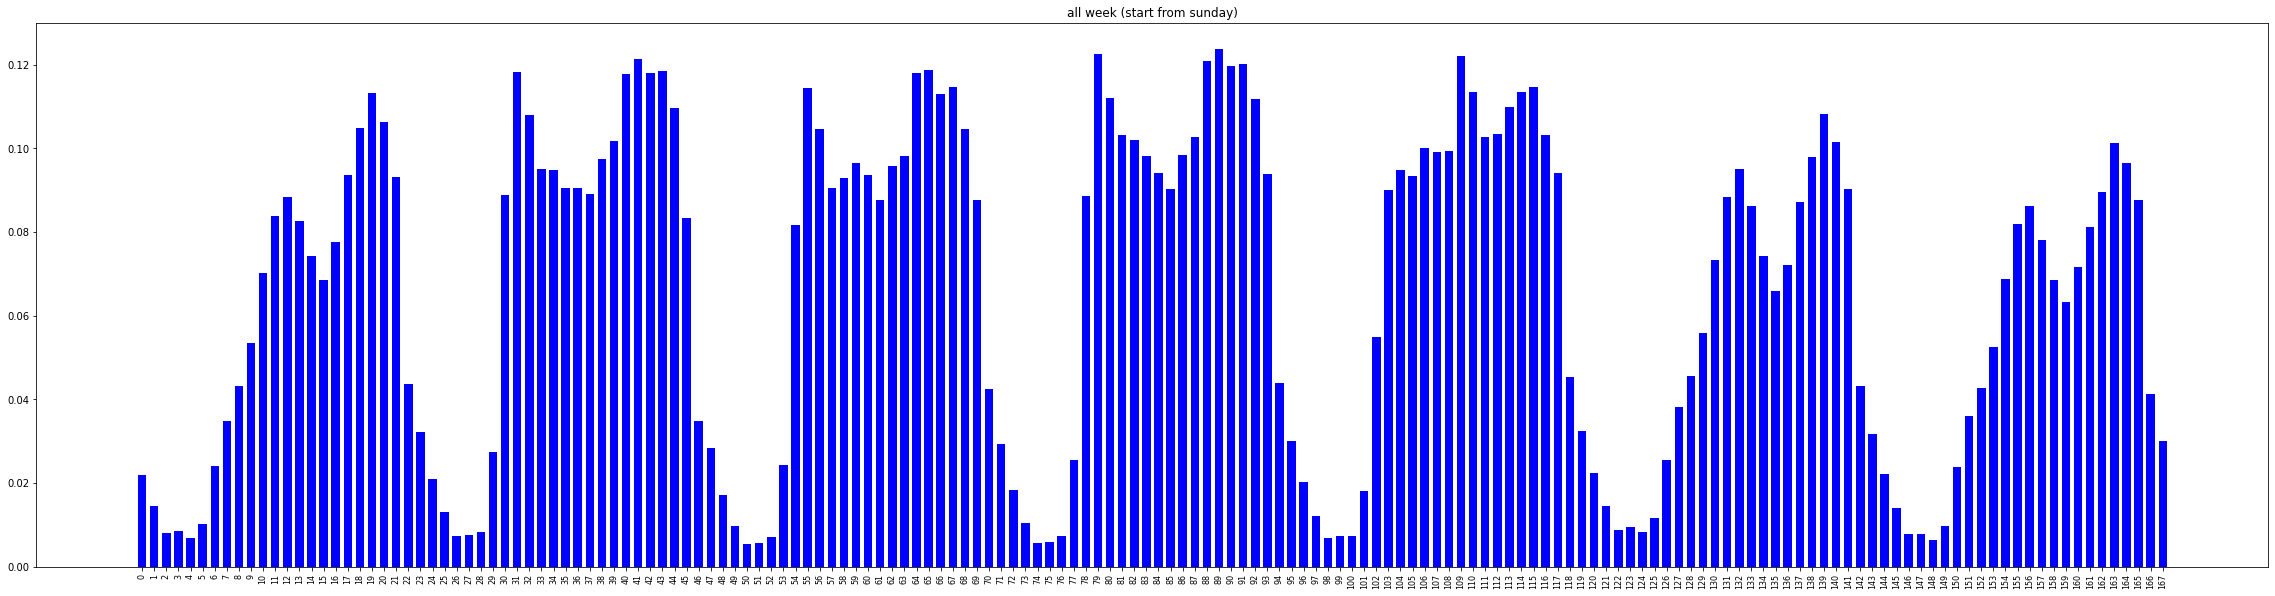
\includegraphics[scale=0.2]{images/HITS/1.png}

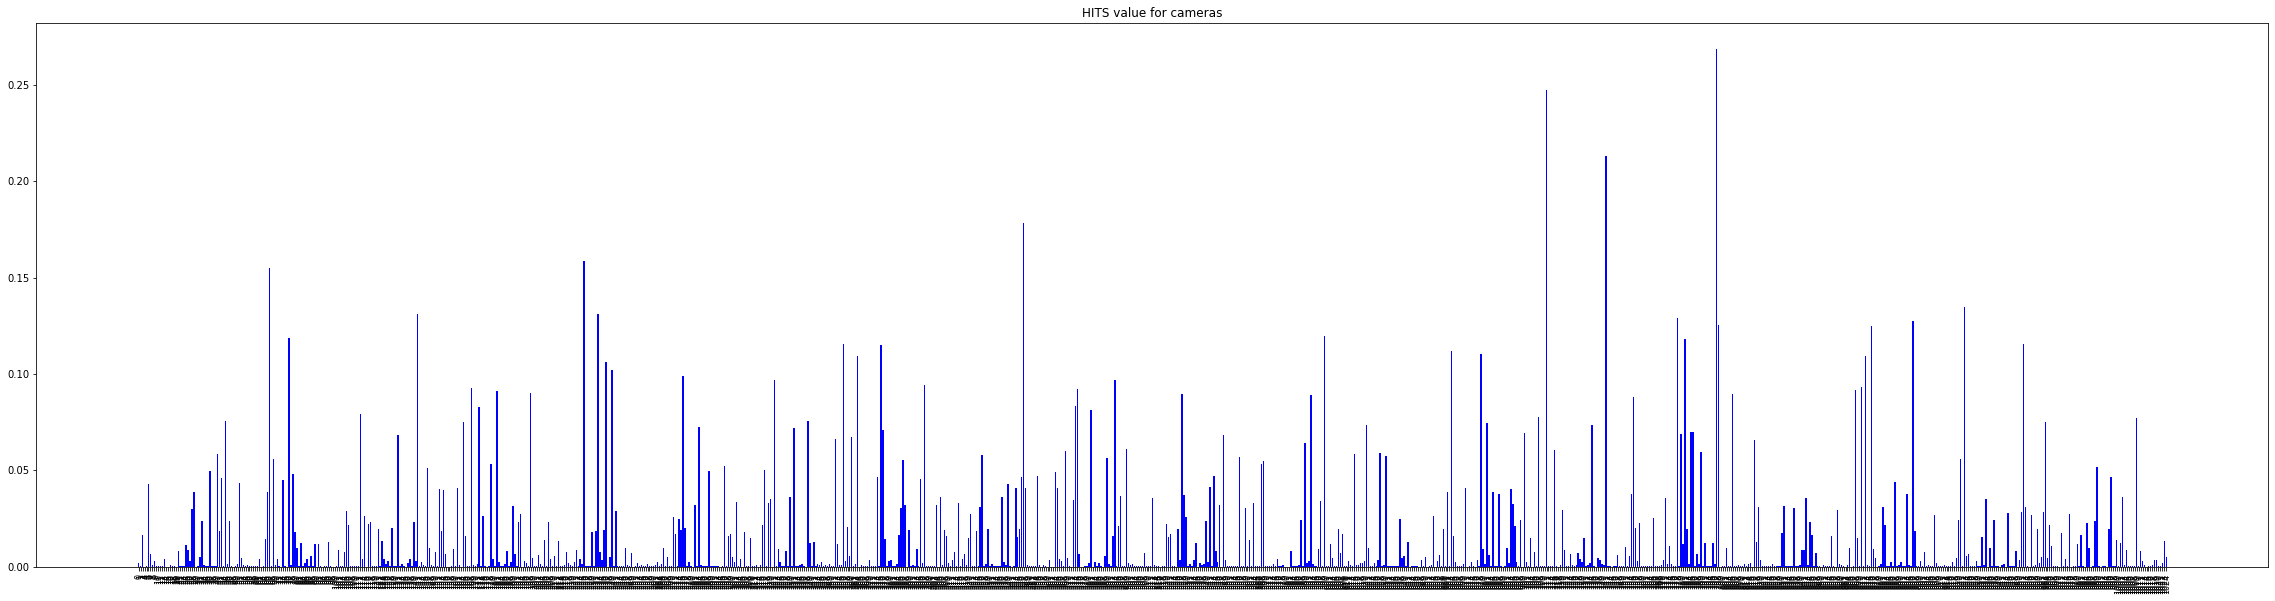
\includegraphics[scale=0.2]{images/HITS/2.png}


\subsection{تحلیل نتایج}
مقادیر این دو نمودار، به ما زمان‌ها یا دوربین‌هایی را نشان‌ می‌دهند که به احتمال بیشتری ثبت می‌کنند. در واقع این نمودار دوربین‌ها می‌تواند 
به ما بگوید که کدام دوربین‌ها در ساعات پرتردد احتمال ثبت بیشتری دارند. اما این اطلاعات خیلی سود‌آور نیست. 
اما در مورد زمان‌ها، نمودار‌ها اطلاعاتی دارند که با شهود ما سازگار است. همانطوری که می‌بینید، روز‌های دوشنبه تا 
چهارشنبه حالت 
U
شکل دارند، که این یعنی دو پیک ترافیکی یکی در صبح و یکی در شب داریم. اما این 
الگو در روز پنج شنبه، احتمالا به دلیل تعطیلی مدارس از بین می‌رود. سپس 
در روز‌های جمعه و شنبه و یک‌شنبه، همانطوری که می‌بینید پیک شب قوی تر بوده است، که دلیل آن 
تعطیلی این سه روز است، که مردم بیشتر در شب تردد دارند (تعطیلی مدارس و ادارات). 


\section{\lr{Important Cameras}}

\subsection{توضیحات کلی}
در این قسمت، سعی کردم از الگوریتم 
HITS
استفاده‌ی بهتری کنم. این بار، راس‌های من تنها شامل دوربین‌ها می‌شوند. کافی است برای هر ماشین 
در هر روز، دوربین‌هایی که پشت هم می‌آیند را یک یال گراف در نظر بگیرم. دقت کنید 
که این یال‌ها جهت دارند. حال اگر از الگوریتم
HITS
استفاده کنیم،‌ می‌توانیم مهم‌ترین مکان‌هایی را پیدا کنیم، که به مکان‌های مهم دیگری مسیر دارند (
    بهترین 
    hub
    ها و 
    authority
    ها
). 

برای انجام دادن این کار، از تابع
lead
در 
sql
استفاده می‌کنیم. برای هر ردیف دوربین‌ ردیف بعدی را به 
df
اضافه می‌کنیم. این کار باید به ازای هر ماشین و هر روز جداگانه انجام شود. 
همچنین باید دقت کنید که داده باید قبل از این قسمت روی زمان مرتب شود (
    lead
    یک سینتکس 
    sql
    است. در صورتی که این قسمت گنگ است، کافی است توضیحات 
    lead
    را بخوانید
). 
نتیجه به صورت زیر شد: 

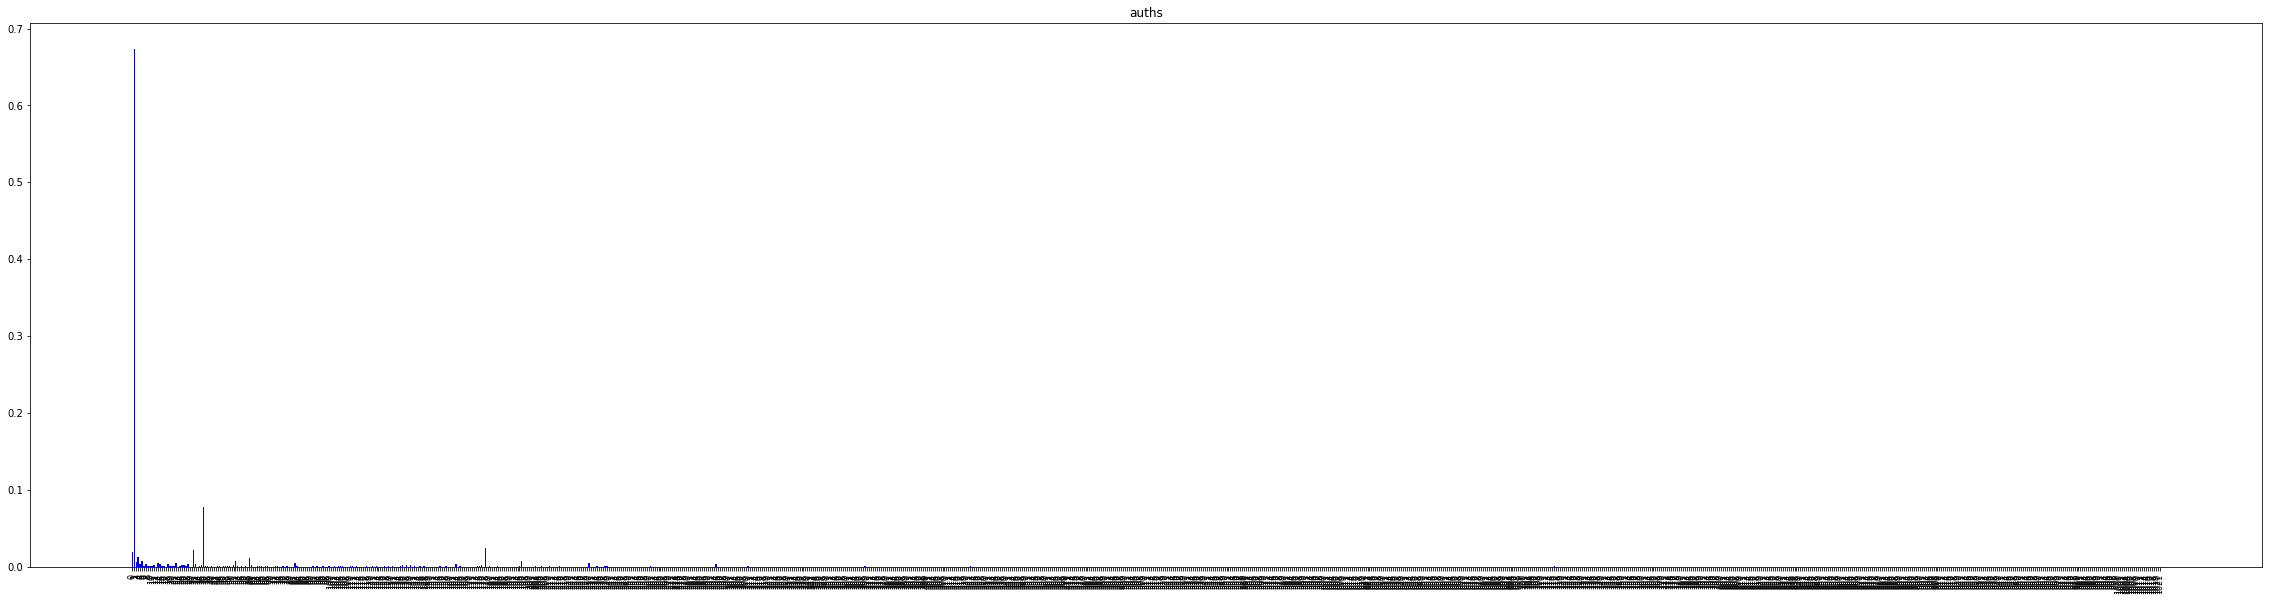
\includegraphics[scale = 0.2]{images/ImportantCameras/1.png}

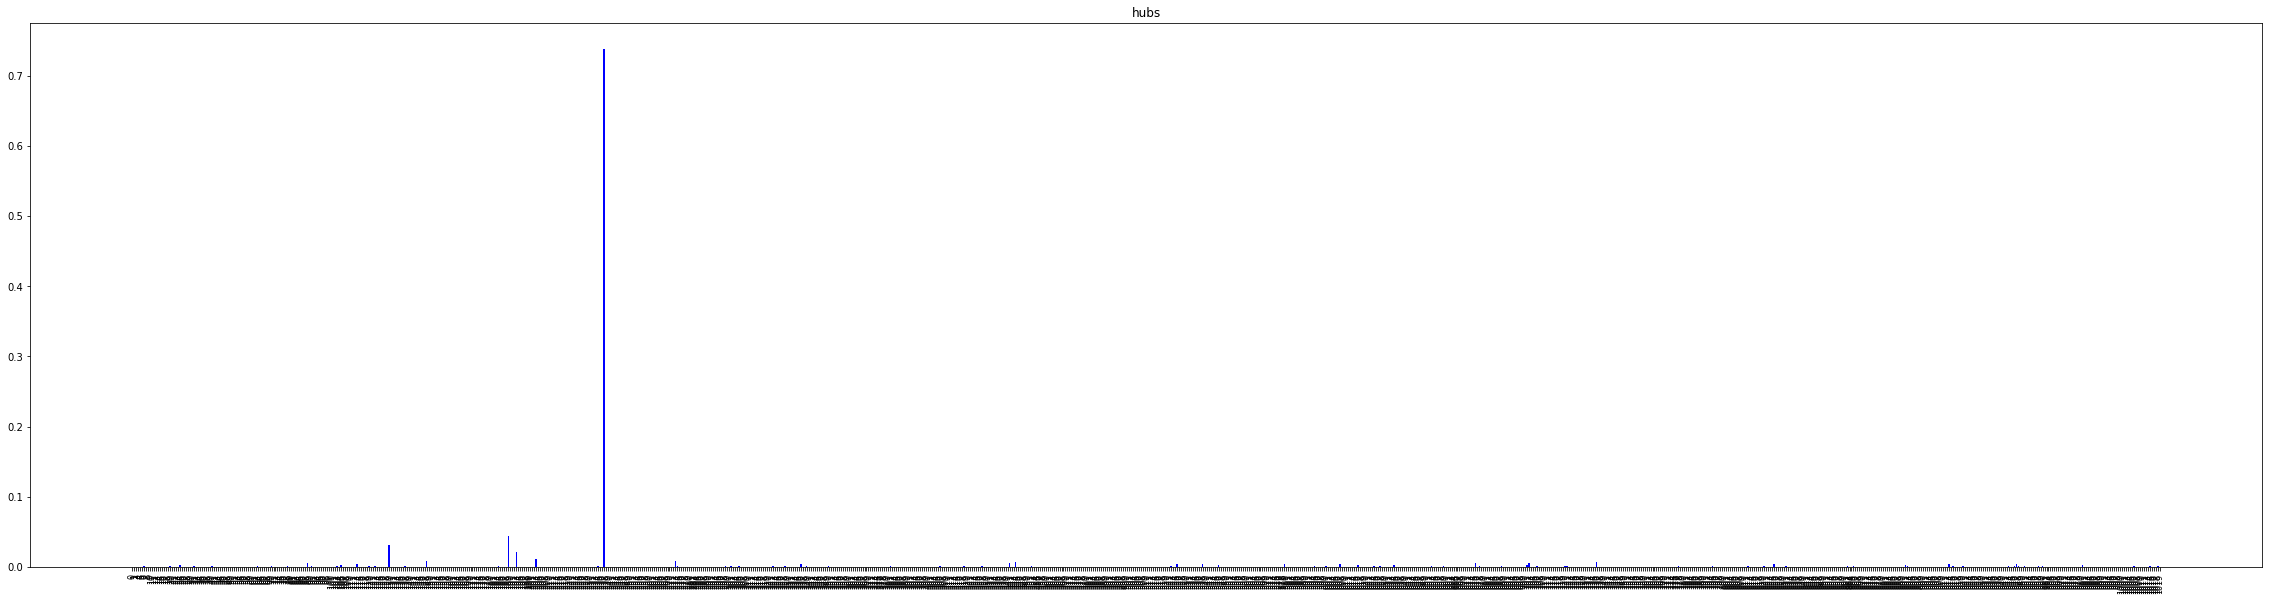
\includegraphics[scale = 0.2]{images/ImportantCameras/2.png}


\subsection{تحلیل نتایج}

همانطوری که می‌بینید، دو دوربین با اختلاف بهترین
hub
و
authority
شدند. لیست این دوربین‌ها به ترتیب در فایل 
jupyter
آمده است (البته دقت کنید که دوربین‌ها اندیس گذاری شده‌اند و اندیس‌ آن‌ها را برنگرداندم). 
نکته‌ی جالبی که وجود دارد این است که با این که دوربین‌ها به ترتیب کل تکرار شدن 
شماره گذاری شده‌اند، اما بهترین 
authority
۴۰ 
مین دوربین پرتکرار ما بوده است (یعنی با این که ۳۹ دوربین از آن پر تکرار تر بوده‌اند، اما بهترین 
authority 
شده است). 


\section{\lr{CF\underline{ }ALS}}

\subsection{توضیحات کلی}

در این قسمت، روشی مانند روش 
\lr{Collaborative Filtering}
به کمک الگوریتم 
ALS
پیاده‌سازی شده است. ابتدا برای هر دوربین و هر ساعت از هفته، تعداد ترددها را به دست آوردم. سپس 
داده را به دو قسمت آموزش و آزمون تقسیم کردم. با کمک داده‌های آموزش مدل 
ALS
را 
train
کردم. سپس با کمک داده‌های آزمون دقت مدل خود را سنجیدم. 

مدل ما قابلیت این را دارد که به عنوان یک 
\lr{Recommender System}
عمل کند. در واقع می‌تواند برای هر دوربین و هر ساعت از هفته، تخمین بزند که چند 
ماشین در دوربین ثبت می‌شوند. کاربرد‌های آن می‌تواند به این صورت باشد که به ما کمک 
کند تصمیم بگیریم آیا یک دوربین در یک زمان خاص نیاز است روشن باشد یا خیر (مثلا 
ممکن است بتوانیم بسیاری از دوربین‌ها را فقط برای چند روز خاص به کار 
بگیریم). 
ممکن است یک دوربین در چند روز ترافیک شدیدی را ثبت کند، در این صورت می‌توانیم 
الگوریتم‌هایی پیش‌نهاد دهیم که به کمک این داده، برای روز‌های بعد مسیر‌های جایگزینی 
به راننده‌ها پیشنهاد دهد. 


\subsection{نتایج}

برای آزمایش مدل خود، علاوه بر توابع آماده که در کد دیده‌ می‌شود، چند دوربین به 
دلخواه انتخاب کردم و داده‌های آنان که در قسمت تست قرار داشت را در نظر گرفتم. 
دقت کنید که مدل ما هیچ وقت این داده‌ها را ندیده‌ است. سپس مقادیر واقعی این داده‌ها 
و مقادیر پیش‌بینی شده را با هم بر روی نمودار نشان دادم. یعنی برای برخی ساعات از روز 
حدس زدم که یک دوربین خاص، احتمالا چند ماشین ثبت می‌کند و 
آن را با مقدار واقعی مقایسه کردم. خطوط قرمز برای داده‌های واقعی و خطوط سیاه مقادیر پیش‌بینی شده هستند. همانطوری که می‌بینید دقت مدل تا حد قابل قبولی بالا است.

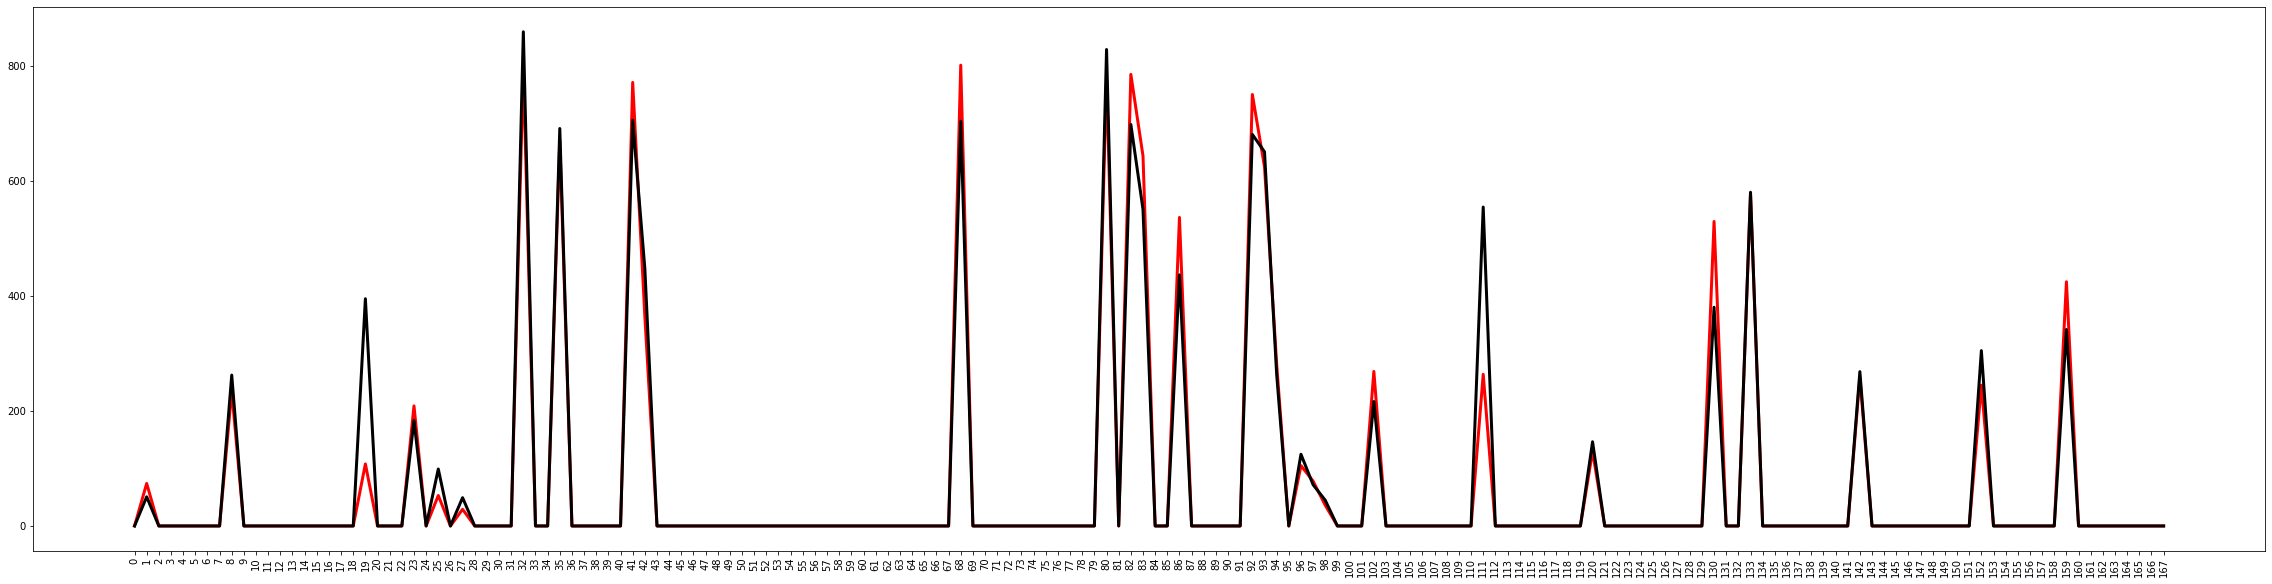
\includegraphics[scale=0.2]{images/CF_ALS/100.png}

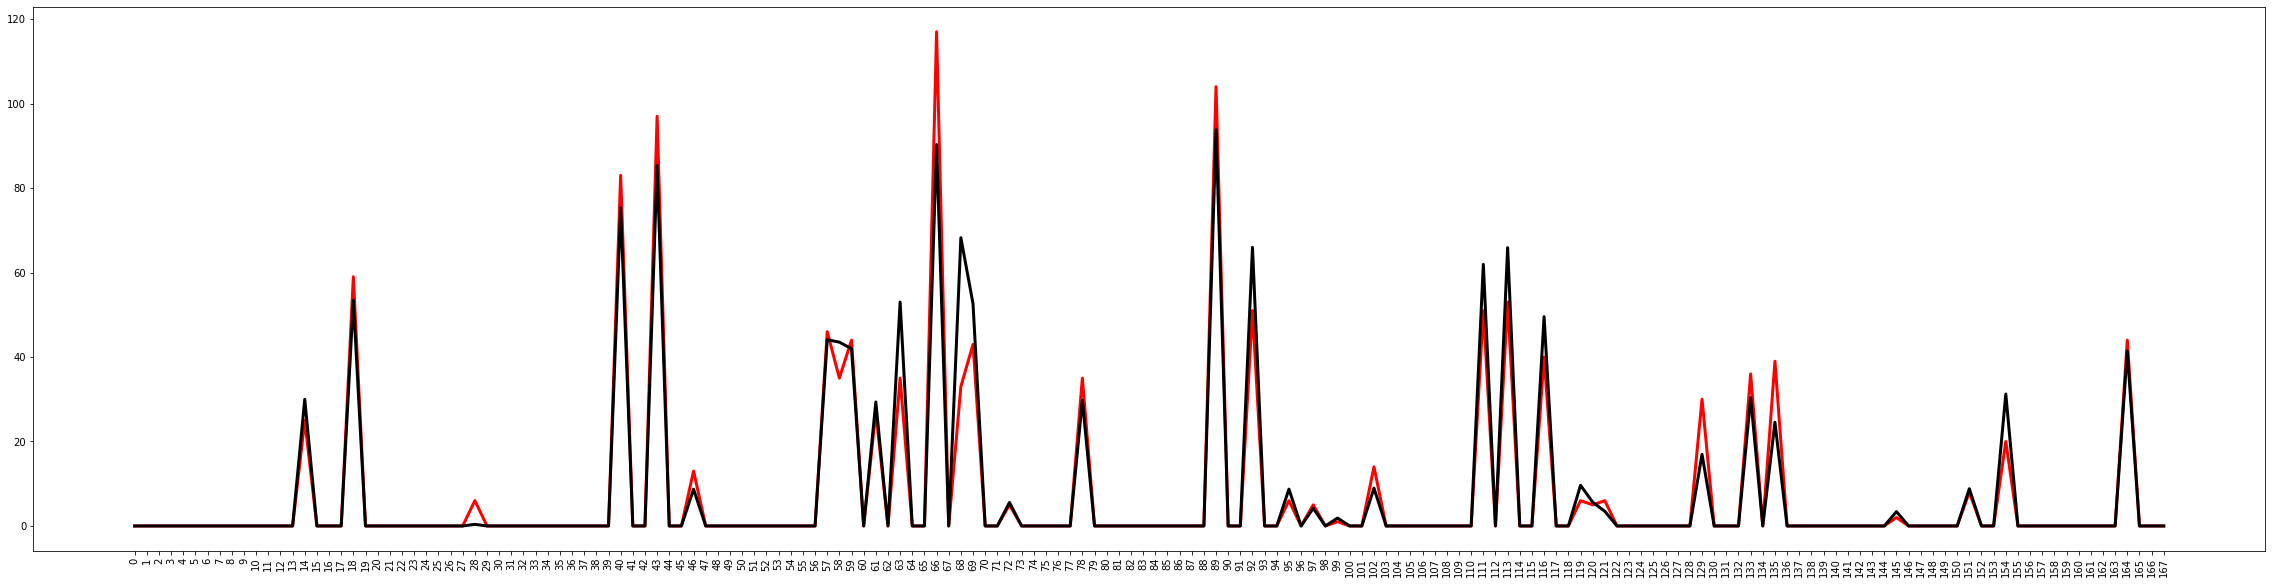
\includegraphics[scale=0.2]{images/CF_ALS/101.png}

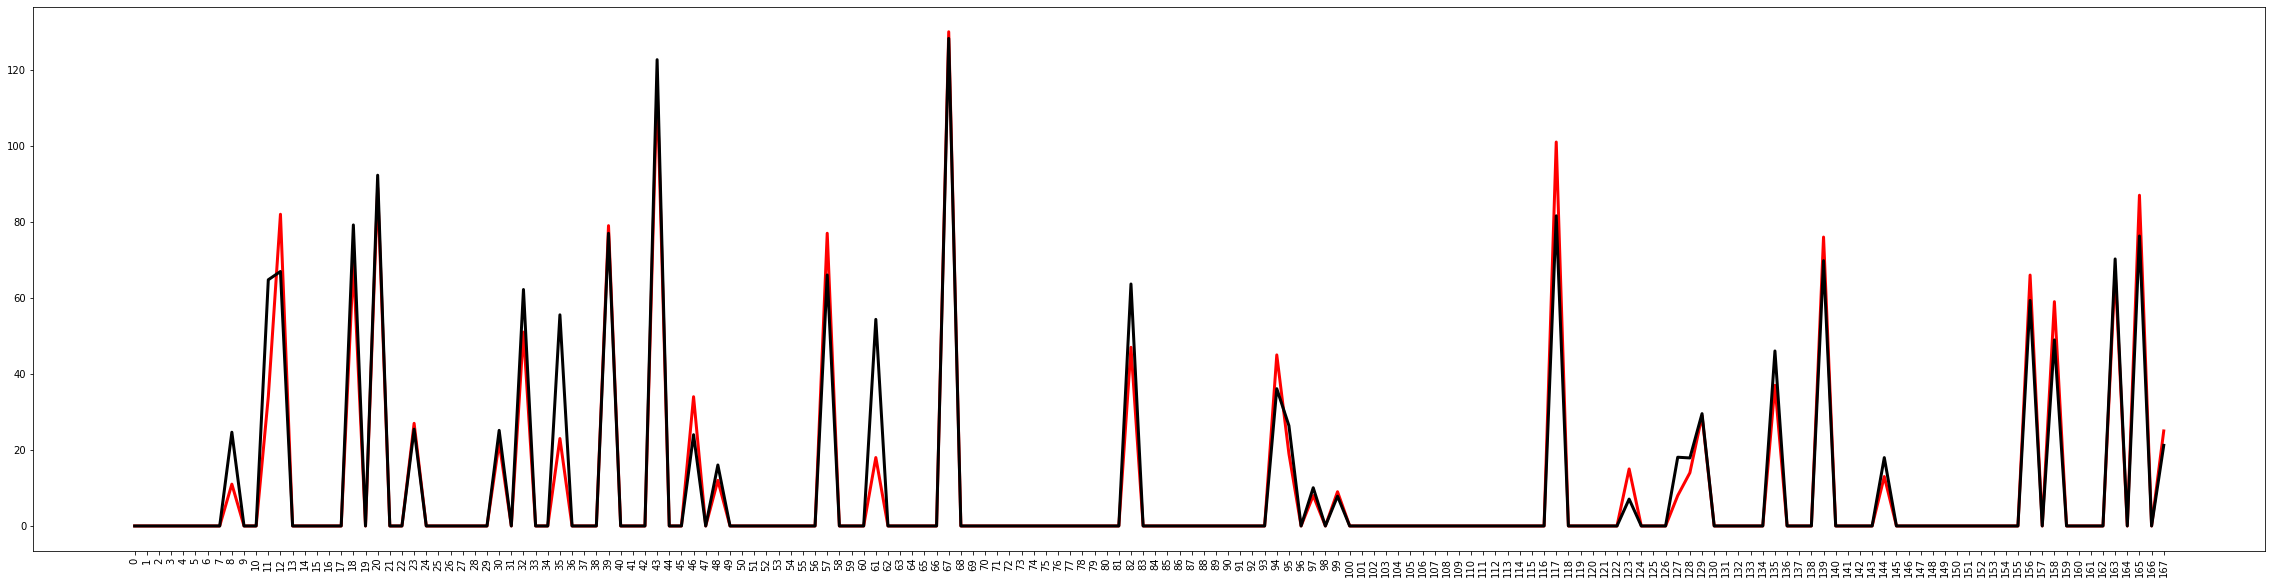
\includegraphics[scale=0.2]{images/CF_ALS/102.png}

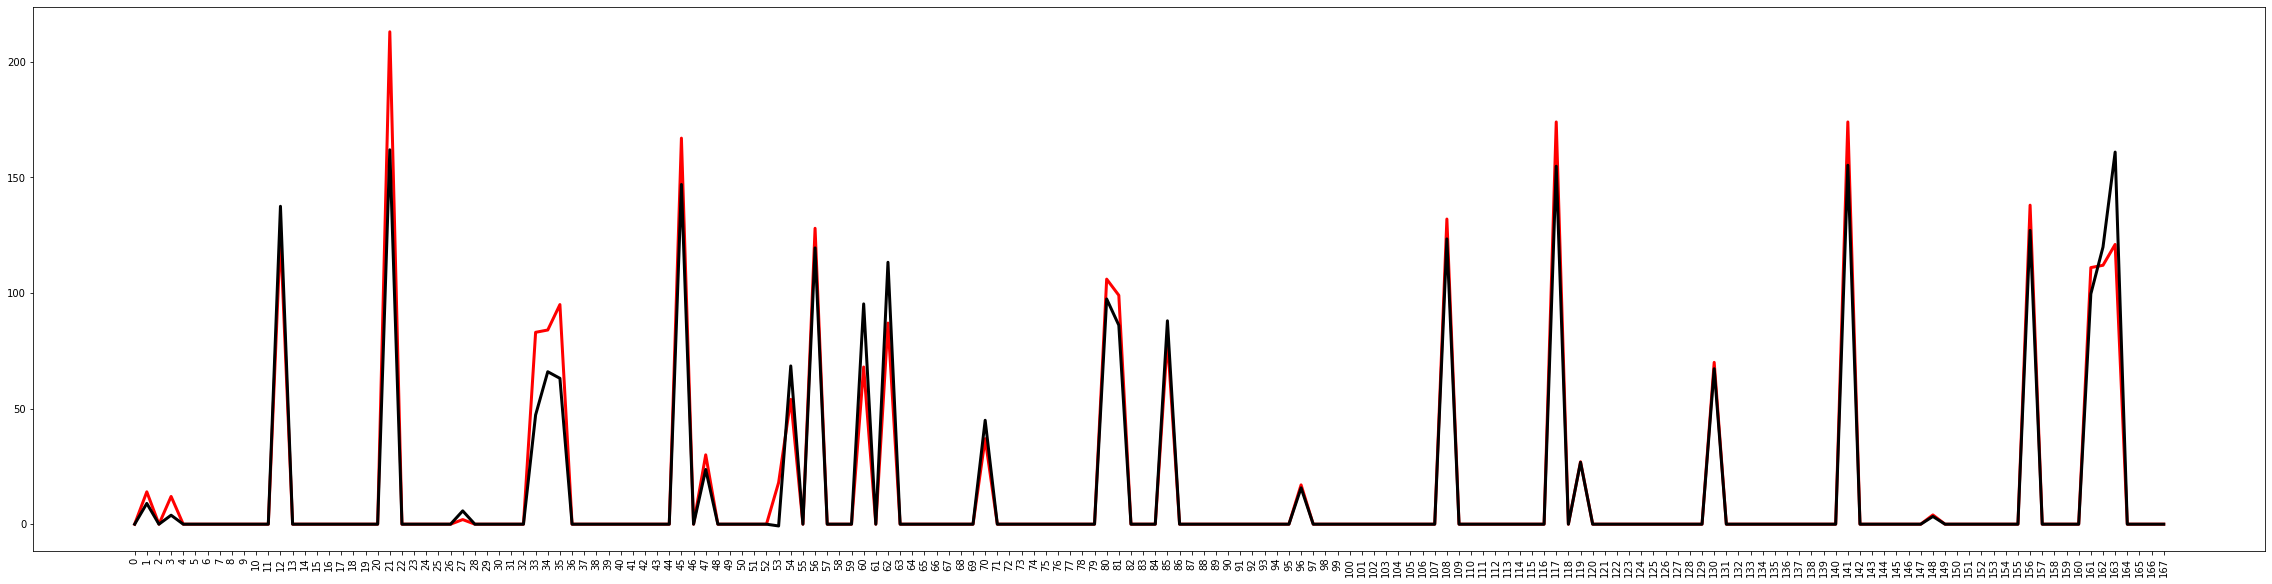
\includegraphics[scale=0.2]{images/CF_ALS/103.png}

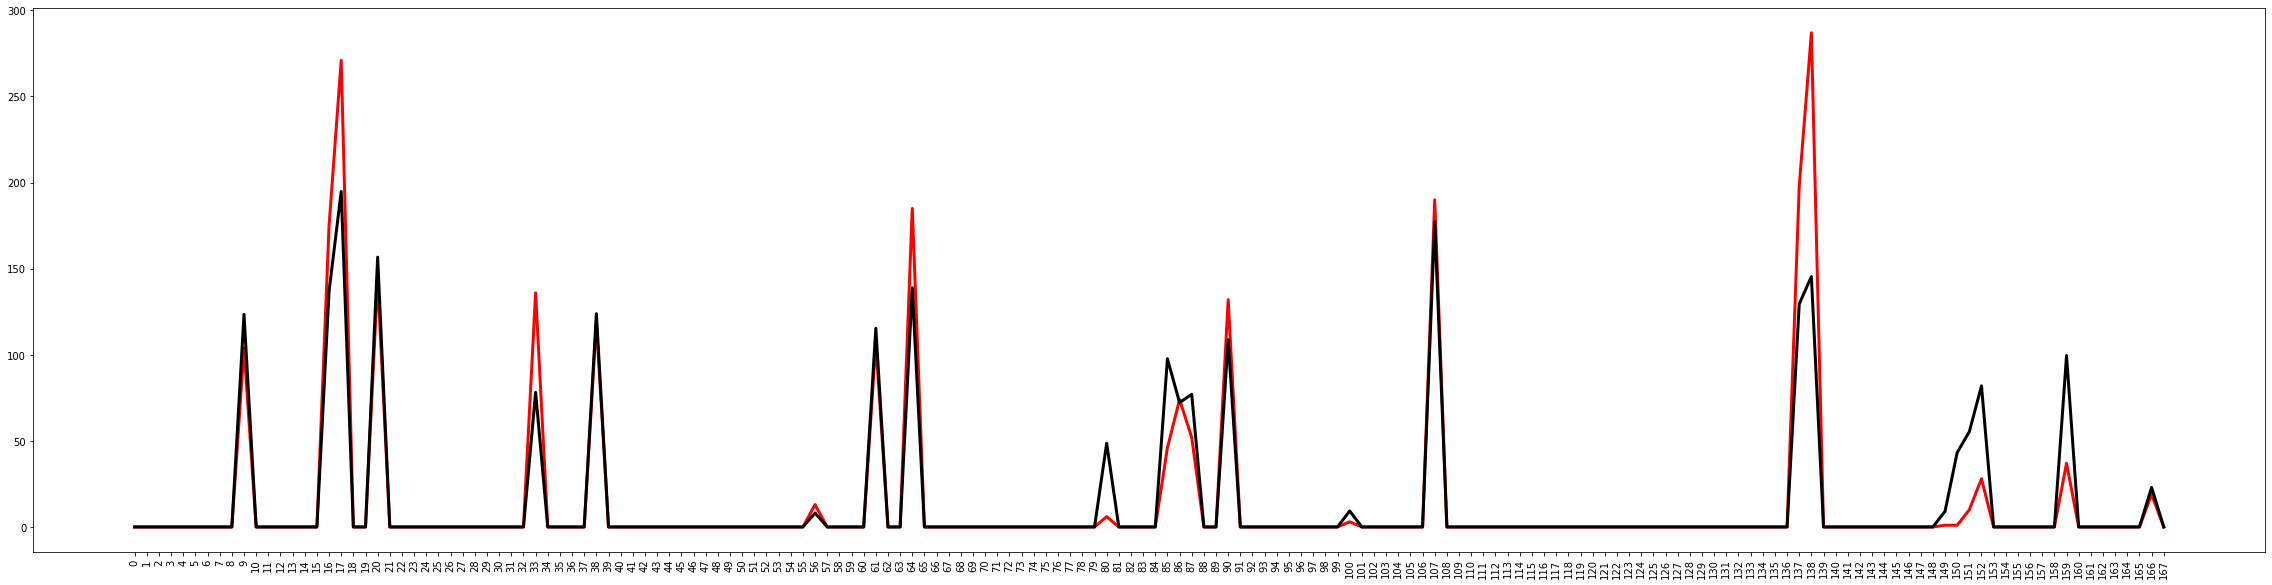
\includegraphics[scale=0.2]{images/CF_ALS/104.png}


\section{SVD}

در این قسمت، ماتریسی ساختم که هر درایه‌ی آن نشان دهنده‌ی تعداد ثبت شدن یک 
ماشین خاص در یک دوربین خاص است. پس از تجزیه‌ی 
SVD
مقادیر منفرد را بررسی کردم تا بتوانم در آن الگویی پیدا کنم. اما 
نتوانستم الگوی مشخصی پیدا کنم و این مقادیر را به مفهوم‌های خاصی پیوند دهم. 
برای تصویر کردن دوربین‌ها و ماشین‌ها روی فضای 
concept 
هم تلاش کردم اما نتیجه قابل فهم نبود. در نهایت بااین که کد این قسمت را 
کامل پیاده‌سازی کردم اما به نتیجه‌ی مطلوبی از نظر مفهومی نرسیدم. 

\end{document}